%\documentclass[a4paper]{article}
\documentclass[T3,WIP]{rapport-iutrs}

\usepackage[utf8]{inputenc}
\usepackage[T1]{fontenc}
\usepackage[francais]{babel}
\usepackage{wrapfig}
\usepackage{graphicx}
%\usepackage[top=2cm, bottom=2cm, left=2cm, right=2cm]{geometry}
\usepackage{eurosym}

\groupe{T306AMAO}
\projet{Gestion d’emprunts bibliothécaires dans une bédéthèque}
\title{Cahier des charges\\Royal}
\auteurs{Steve Benedick\\Jean Meyblun\\Kévin Hagner}
\livrable{Cahier des charges} 
\version{1.0}
\date\today

\begin{document}

%\maketitle
\pagedegarde 

\newpage{}
\part*{Introduction}
Notre projet à pour but la gestion informatique des emprunts et achats de bandes dessinées (bd) réalisé par un particulier.
Pour cela nous allons partir d'une application existante, \emph{Royal}
\footnote{Site officiel du projet Royal : www.royal-project.org}, qui permet la saisie et l'enregistrement de bandes déssinées, et l'améliorer.
En effet, Royal ne permet qu'une saisie manuelle de chaque ouvrage, et ne gère ni les bibliothèques d'emprunt ni les dates d'emprunt et de retour. Ainsi nous allons ainsi permettre à un utilisateur de simplifier sa gestions de bd, d'une part en améliorant l'application Royal et d'une autre part en développant une application mobile pour Android.

L'amélioration consistera en :
- l'automatisation de l'ajout d'une bd grâce à son code barre qui permettra la recherche et le remplissage automatique de l'ensemble des informations de l'ouvrage,
- l'ajout d'un système de bibliothèque, de durée d'emprunt, de date d'emprunt, tout cela pour pouvoir notifier à l'utilisateur s'il doit penser à rendre certains de ses ouvrages, d'où proviennent ses ouvrages et combien de temps il lui reste pour les lire,
- la synchronisation avec l'application Android.

L'application Android doit permettre :
- La capture des codes barres d'un ensemble de bd
- l'envoie des codes barres à l'application améliorée de Royal qui grâce à la synchronisation sera capable d'ajouter automatiquement un lot de bd

Le projet est à but personnel, il n'a comme unique objectif que de servir d'aide mémoire à un utilisateur.
Il ne s'agit par exemple pas d'un système de gestion de bibliothèque ou de stocks des bd restantes dans une librairie.
Aucunes relation ne sera possible entre différents utilisateurs, ni de mises en commun des œuvres lues
(statistiques des livres les plus lus par la « communauté », notation, commentaires…).

\newpage{}

\tableofcontents
\newpage{}

\part{Définition des fonctionnalités}
Cette partie liste toutes les fonctionnalités attendues dans le programme. Celles-ci sont classées par priorité.

\begin{description}
\item [Priorité 1 :]
	Priorité la plus élevée. Il s'agit des premières fonctionnalités à implémenter permettant au logiciel de répondre à la demande de base de l'utilisateur.

\item [Priorité 2 :]
	Éléments nécessaires, ceux-ci serons effectués dans un second temps. Il s'agit d'améliorations du programme de base, qui permettent d'optimiser le programme afin de répondre aux autres demandes du client.  

\item [Priorité 3 :]
	Éléments secondaires. Ces fonctions ne sont pas demandées, mais ajoutent une plus-value au programme. 
\end{description}


\section{Relatives au client PC}

\subsection{Système d'ajout et d'édition de bande dessinées}
\paragraph{Ajout des information de bases ---  \textit{Priorité 1}:}
C'est une des fonctions sans laquelle le projet n'a pas lieu d'être. Elle est à la base de la gestion des \emph{BDs}. En effet, cette fonctionnalité permet l'ajout, la sauvegarde et l'édition de l'ensemble des informations des albums qui pourront être ajouté dans l'application. Ces informations correspondent par exemple, au titre, à l'auteur, au genre, etc... d'un album.

\paragraph{Création de liens entre les albums ---  \textit{Priorité 1}:}  
Cette fonction doit permettre de créer des liens entre les différents albums, s'il partage des informations en commun, comme leur auteur, ou leur genre.

\paragraph{Ajout d'une image de couverture ---  \textit{Priorité 2}:}  
Cette partie devra également être capable d'associer une image à l'album pour permettre de visualiser sa couverture.

\subsection{Système d'affichage des \emph{BDs} selon certains critères}

\paragraph{Affichage des \emph{BDs} ---  \textit{Priorité 2}:}

La visualisation d'une liste d'albums parait nécessaire pour l'utilisateur afin gérer sa bibliothèque personnel. Ainsi, l'application devra comporter cette visualisation qui sera paramétrable par l'utilisateur voulant faire une recherche spécifique, par exemple une recherche par auteur ou par genre.

\subsection{Système de recherche d'informations sur une \emph{BD}  grâce au code barre}

\paragraph{Saisie et vérification du code barres ---  \textit{Priorité 1}:}
Dans un premier temps, cette fonction doit permettre la saisie d'un code barres par l'utilisateur. 
Celui-ci doit être vérifié par l'application. En effet, il est possible de l'analyser pour savoir s'il correspond bien à un livre et dans un second temps d'en extraire son code \emph{ISBN}, code représentant de manière internationale le livre.
\paragraph{Recherche d'informations grâce au code barres ---  \textit{Priorité 1}:}  
Un fois le code analysé, l'application effectue une recherche sur une base de données externe des informations sur l'album et sera capable de les ajouter automatiquement dans l'application.
\paragraph{Traitement en fonctions des résultats de la recherche ---  \textit{Priorité 1}:}  
Le système sera capable de gérer le cas où le code barres n'est pas valide ou si les informations à récupérer sont inexistantes ou incomplètes.

\subsection{Système d'importation des albums}
\paragraph{Importation via courriel ---  \textit{Priorité 1}:}
L'application devra pouvoir importer des albums. 
Ceci est en étroite liaison avec l'application Android. Il est nécessaire de définir un protocole d'échange entre les deux applications. Nous allons donc présenter cette partie sous l'aspect d'un échange de courriel, solution certes non optimale mais qui a l'avantage d'être indépendant de tout autre système distant souvent couteux.

\subparagraph{Configuration de l'adresse du courriel :}  
Ainsi en considérant l'échange via mail, l'application devra intégrer un système de configuration d'adresses courriel pour permettre à l'utilisateur de choisir à partir de la quelle il souhaite récupérer les albums.

\subparagraph{Réception des courriels spécifiques :}  
L'application devra dans un second temps lire et reconnaitre les mails spécifiques reçus dans la boite à courriel du compte et pouvoir en retirer les albums qu'elle contient.

\subparagraph{Ajout automatique des albums récupérés :}  
Finalement l'application pourra ajouter automatiquement les albums, un par un ou par lot (Voir : Système d'envoi sur Android). 
Pour le contenu des courriels, il pourrait ne s'agir que de leur code \emph{ISBN}, puis par la suite lors de l'importation, une recherche sur les systèmes d'informations distant permettra de compléter les informations à insérer.
\paragraph{Importation via un autre moyen ---  \textit{Priorité 3}:}  
L'ajout d'un autre moyen d'importation est aussi à étudier, par exemple via bluetooth ou via USB avec un smartphone Android.

\subsection{Système de gestion des lieux et dates d'emprunt}
\paragraph{Bibliothèques et dates de retour ---  \textit{Priorité 2}:}
Que ce soit lors d'un import, ou simplement lors d'un ajout manuel, l'utilisateur pourra ajouter, si son album ou son lot est issus d'un emprunt bibliothécaire, et, si oui, d'une date de retour. 
Il pourra par la suite trier ses albums en fonction de ces informations.

\paragraph{Système d'alerte pour les dates de retour ---  \textit{Priorité 3}:}  
L'application possèdera un système de configuration pour permettre à l'utilisateur d'être notifié s'il doit rendre ses livres. Ces notifications surviendrons, ou non (l'option sera désactivable) un certain nombre de jours (configurables) avant la date de retour.



\section{Relatives au client Android} 


\paragraph{}
Afin de faciliter la saisie des code barres des différents albums, une application Android sera développée afin de capter les différents code barres et les transmettre au client PC.

\subsection{Système de capture des code barres}
\paragraph{Capture unique ---  \textit{Priorité 1}:}
Afin de récupérer les code barres sur les différents albums nous développerons une fonction permettant de les capter à l'aide de l'appareil photo.
Pour les récupérer, il suffira de placer le code-barre devant l'objectif de l'appareil photo du mobile pour qu'il soit reconnu.

\paragraph{Capture multiple ---  \textit{Priorité 1}:}
Tout comme le mode de capture unique, cette fonction permettra de capter les codes barres mais cette fois ci, c'est toute une série qui pourra être capturée afin d'envoyer tous les codes barres en même temps \textit{(Voir fonction système d'envoi des albums)}

\subsection{Système d'envoi des albums}
\paragraph{Envois par mail ---  \textit{Priorité 1}:}
\subparagraph{Configuration d'une adresse :}
Afin de permettre l'envoi des albums par courriel \textit{(voir Système d'envoi par courriel)}, une fonction permettant de configurer les différentes adresses utilisables est nécessaire. (L'adresse utilisée pour l'envoi, sur l'application Android doit être la même que celle du client PC).

\subparagraph{Système d'envoi par courriel :} 
Une fois les codes barres captés, une fonction permettra au client Android de les envoyer au client PC. 
Le mail aura une syntaxe spéciale afin d'être reconnue et analysée plus facilement par le client PC. 

\paragraph{Envoi par un autre moyen ---  \textit{Priorité 3}:}
Certains utilisateurs n'ayant peut-être pas de connexion internet avec leur forfait mobiles ou n'y ayant pas accès (lieu isolé non desservie par les reseau mobile ou pays étranger), une fonction permettant l'envoi des albums via un autre moyen que le courriel pourra être développé.
Exemples de moyen pouvant être étudié afin de permettre cet envoi: Bluetooth, USB…

\subsection{Vérification de la validité du code barres}
L'application vérifiera si les code barres captés sont bien associés à un livre.
Si c'est le cas, l'\emph{ISBN}, ainsi que le titre du livre seront affichés à l'utilisateur.
Si le code barres ne correspond pas à un livre, l'utilisateur en sera averti via un message d'erreur.

\subsection{Système d'enregistrement des albums déjà scannés}
\paragraph{Enregistrement des albums ---  \textit{Priorité 2}:} 
Afin d'empêcher l'envoi d'albums déjà captés, leurs \emph{ISBN} seront enregistrés dans l'application Android. 
De cette façon, l'utilisateur pourra être avertis en cas de capture d'un album déjà scanné.
Il lui sera cependant permit de renvoyer l'album s'il le désir.

\paragraph{Mise en commun avec les albums du client PC ---  \textit{Priorité 2}:} 
Comme il sera possible à l'utilisateur d'ajouter des albums sur le client PC sans passer par le client mobile, il sera possible de mettre en commun les albums enregistrés sur le client Android avec les albums disponibles sur le client PC.
Lors de cette mise en commun seul les albums présents sur le client PC seront gardés sur le client Android et tout autre album non présents sur le clients PC sera supprimé.  


\newpage{}

\section{Utilisation type}
Dans cette partie sera évoqué une description du processus de fonctionnement du programme.

\subsection{Lancement de l'application Androïd}

\paragraph{Captation d'un unique ouvrage} 


Si l'utilisateur choisi le mode de capture unique, alors le programme vérifie si l'adresse courriel est configurée ou non. 
Si elle ne l'est pas, alors le programme lance le processus de configuration. 
Une fois certain que celle-ci est correctement configurée, la phase de capture réelle est exécutée. 
Si l'\emph{ISBN} retourné est valide, alors le client Android envoie les informations sur le client PC. 
Si ça n'est pas le cas, il proposera à l'utilisateur de refaire une capture. 


\begin{figure}[htbp]
  \begin{center}
    \leavevmode
    \subfloat[Menu de l'application Royal\_Scanner]{%
		\label{}
		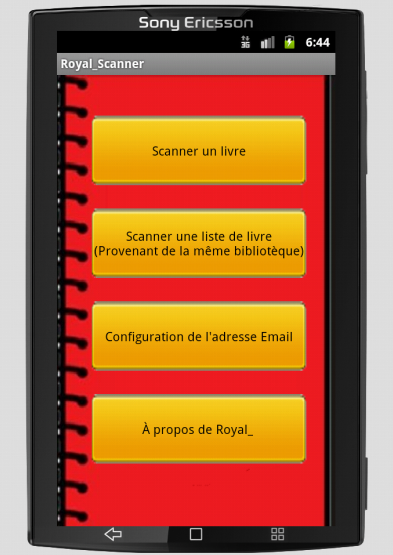
\includegraphics[height=7cm]{../img/Royal_Scanner_menu.png}}
    \hspace{4cm}
    \subfloat[Phase de capture du code barre]{%
		\label{}
		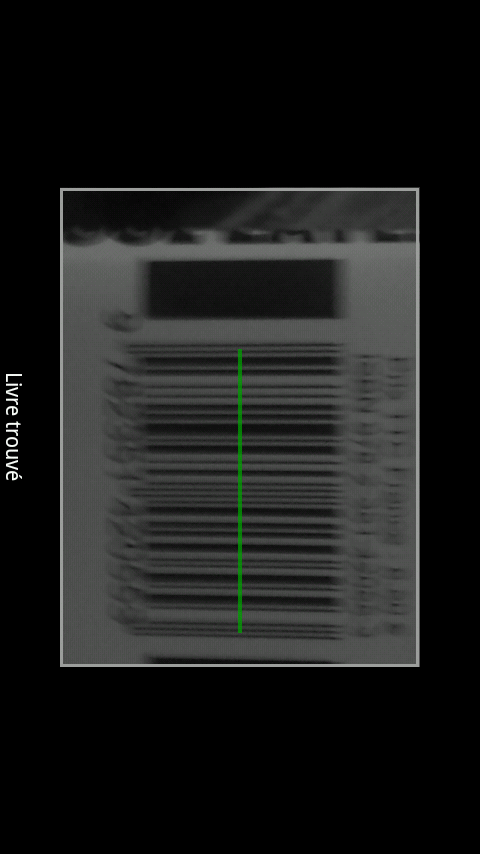
\includegraphics[height=7cm]{../img/Royal_Scanner_prisescanner_2.png}}
  \end{center}
\end{figure}

\paragraph{Capture d'un lot d'ouvrages}
Si l'utilisateur choisi de capturer directement plusieurs \emph{BDs}, alors le programme exécutera en boucle le processus utilisé pour une simple \emph{BD}. 
Le seul changement interviendra après la validation de la bonne capture de l'\emph{ISBN} :
Il sera en effet demandé à l'utilisateur si celui-ci désire continuer la capture ou d'y mettre fin. 

Si il choisi d'y mettre fin, alors les informations seront transmises au client PC. 
Si au contraire, il choisi de continuer la capture, alors le programme rebouclera. 

\subsection{Lancement de l'application PC}


\begin{wrapfigure}[5]{r}[1cm]{5cm}
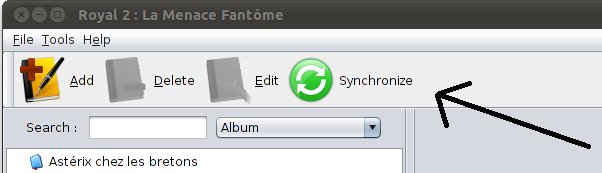
\includegraphics[width=5cm]{../img/btn_synchro.png}
\caption{Bouton d'importation}
\end{wrapfigure}
\paragraph{Importation des livres}
Si l'utilisateur choisi d'importer les livres. Alors le programme teste si l'adresse courriel est correctement configurée. Si ce n'est pas le cas, le processus de configuration est exécuté. 

Une fois que le programme a une configuration de courriel valide, celui-ci y recherche les messages présents à son attention. 

\begin{wrapfigure}[12]{r}[1.5cm]{8cm}
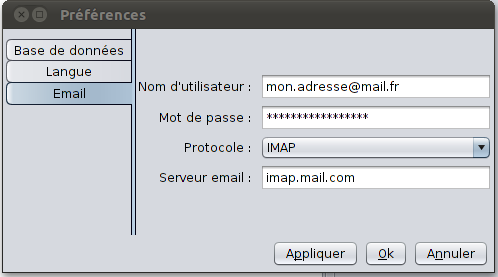
\includegraphics[width=8cm]{../img/preferenceMail.png}
\caption{Configuration du mail}
\end{wrapfigure}
\paragraph{Importation des livres}
Tant qu'il y a des messages à l'attention du programme, celui-ci les lit. 
Tant que des numéros d'\emph{ISBN} sont présents dans le courriel, ils sont récupérés. 
Une fois tous les \emph{ISBN} récupérés, le programme recherche des informations sûr les livres sûr internet.
L'utilisateur peut ensuite modifier ces données, puis peut renseigner les informations relatives à la bibliothèque. 

Si la bibliothèque dans là quelle le livre (ou le lot) a été emprunté existe déjà, 
alors l'utilisateur n'aura qu'à la choisir dans une liste. Si elle n'existe pas encore, elle pourra être rajoutée via une fonction disponible. 
Enfin, l'utilisateur pourra indiquer la date de retour maximale du livre (ou du lot).

\paragraph{Vérification de la date de retour}
À chaque lancement de programme, les dates de tous les ouvrages encore en possession de l'utilisateur seront testés afin de voir si l'ultimatum n'est pas arrivé à terme. 
Les noms de tous les livres ainsi repérés sont conservés puis affichés à l'utilisateur une fois la recherche terminée. 


\begin{wrapfigure}[12]{l}[1cm]{8cm}
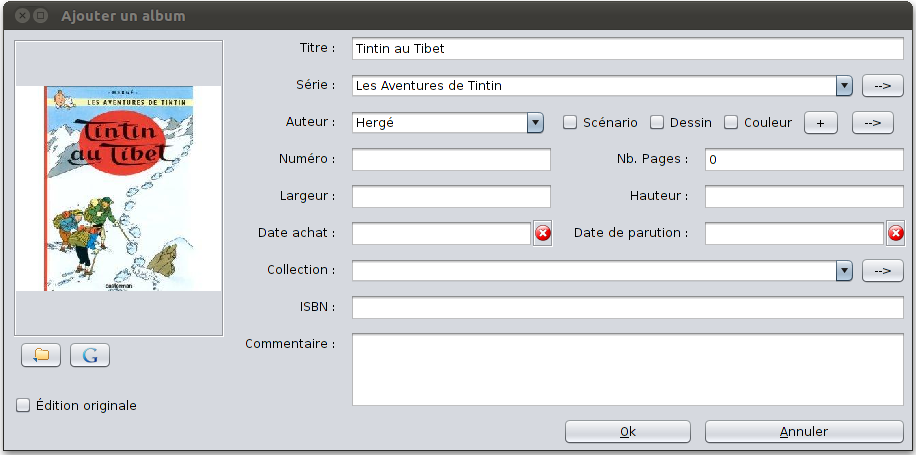
\includegraphics[width=8cm]{../img/editionAlbum.png}
\caption{Edition d'un Album}
\end{wrapfigure}

\paragraph{Modification des information d'un livre}
Si l'utilisateur souhaite modifier des informations sur un livre enregistré dans le programme, il pourra visualiser les albums par critères tels que l'auteur, la collection, le type…
Une fois le livre sélectionné, il faudra cliquer sur le bouton « éditer ».  
C'est à ce moment que l'utilisateur verra apparaitre les différentes informations sur le livre et pourra les modifier.
Une fois satisfait des changements, l'utilisateur pourra soit valider les modifications, soit les annuler. 
En cas de validation de la modification, le programme enregistrera les nouvelles informations dans la base de données.  

\newpage{}

\part{Analyse de l'existant}


\section{Fonctionnement de l'application Royal}

Comme nous pouvons l'observer le MCD existant n'est pas parfaitement obtimisé et certaines des informations ne sont jamais utilisé dans l'aplication Royal. 

\subsection{Introduction}
Nous n'avions pas d'existant imposé à proprement parlé, cependant nous avons été guidé vers Royal, un projet existant réalisé par des étudiants du département informatique l'an passé.
Il apparait être une des solutions actuelles la plus en accord avec la demande client à savoir de manière générale, « la facilitation de gestion d'une bédéthèque ».

De ce fait, cet article traitera du fonctionnement de Royal.
Royal est une application 
libre \footnote{Selon les termes de la GNU Lesser General Public License}
issus d'une amélioration de Birdy, une autre application libre de gestion de livre.

\subsection{Aspect fonctionnel de Royal}
Royal permet la saisie d'informations sur une bande déssinée (BD), tel que son titre, son auteur, son image de couverture (recherchée sur internet), sa date de parution, etc..
Il permet d'obtenir une liste de l'ensemble des BDs, que l'on peut trier selon divers critères et réorganiser selon des collections de BDs.
Royal permet l'enregistrement de BDs, mais aussi d'informations concernant les auteurs ou encore les collections.
L'on peut aussi importer un ensemble de BD à partir d'une base de donnée existante.
De plus Royal intègre un système multilangue concernant son interface utilisateur, ainsi que d'une bibliothèque d'aide d'utilisation.

\subsection{Aspect technique de Royal}
Royal est développé en Java et utilise la bibliothèque \emph{Swing} pour son environnement graphique. 
Le projet à été développé sous Linux, mais reste néanmoins éxécutable sous d'autres systèmes d'exploitations comme Windows 7 par exemple, avec plus ou moins de succès. 
L'ensemble des données stockées est fait via \emph{Hibernate}, c'est un framework gérant la persitance des objets en base de données. 
C'est un outil lourd et complexe mais très puissant que nous allons réutiliser étant donné sa mise en place existante sous Royal qui permet un transfert simplifié entre objets java et base de données.

\subsection{Analyse de la base de données déjà existante}
\begin{figure}[h]
\begin{center}
 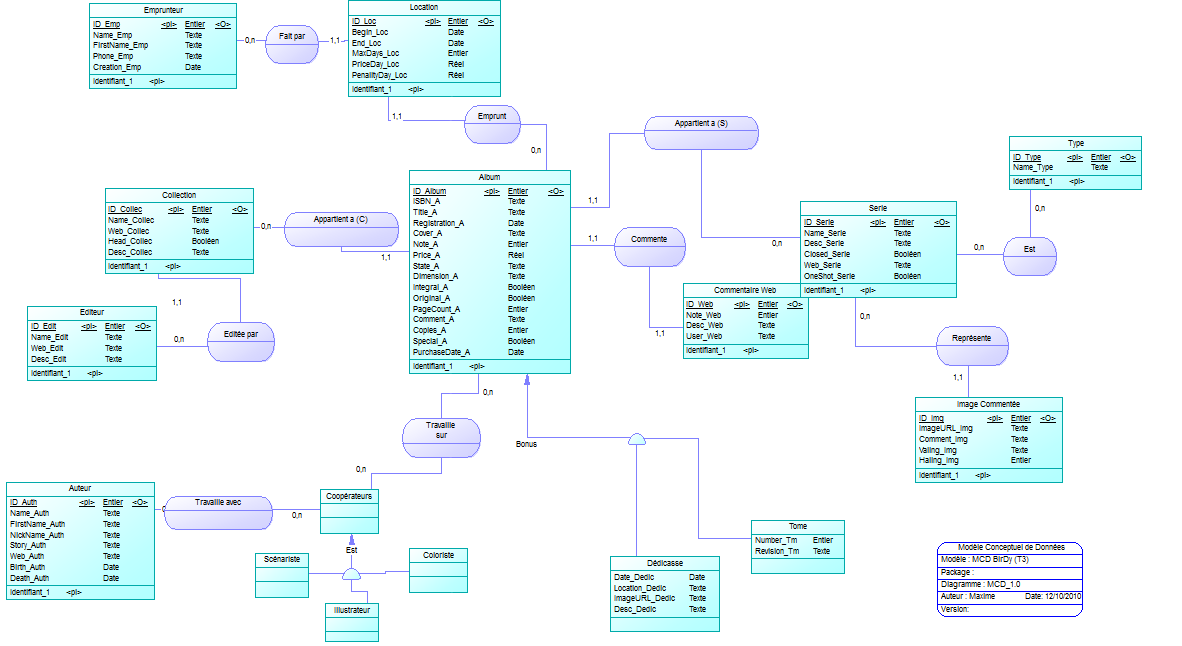
\includegraphics[height=6cm]{../img/MCD_Royal.png}
\end{center}
\caption{MCD Repris de la documentation déjà existante de Royal}
\end{figure}

\newpage{}

\part{Planning prévisionnel}

\section{Étapes du projet}

Notre projet comporte 4 étapes principales. Chacune de ces étapes aura une date de remise définie dès le début du projet. 

\paragraph{La rédaction du cahier des charges}

Dans cette étape, nous avons principalement eu besoin de rédiger la demande du client. 
Nous avons aussi eu à étudier le fonctionnement du logiciel Royal que l'on a choisi d'améliorer afin d'arriver au but visé.
Les contraintes liées à l'amélioration de ce logiciel nous permettent de définir la faisabilité des différentes fonctions. 

\paragraph{La rédaction du dossier d'analyse}

Dans cette partie, nous aurons à approfondir l'analyse ainsi que la conception des différentes fonctions et le fonctionnement du logiciel Royal. 
Nous définirons aussi les différents outils utilisés afin de développer le projet, tel qu' 
Eclipse \footnote{Site de l'IDE Eclipse : http://www.eclipse.org/} 
pour le développement JAVA, ou encore 
PowerAMC \footnote{Site officiel de PowerAMC : http://www.sybase.fr/products/modelingdevelopment/poweramc}
pour la réalisation des MCD.

\paragraph{La réalisation d'un premier prototype}

Afin de rendre un prototype le 5 Décembre 2011 répondant aux principales demandes de l'utilisateur, nous développerons les fonctions de priorités 1 et 2.
Pour permettre l'implémentation de certaines de ces fonctions, nous aurons à modifier la base de données en suivant le modèle modifié dans l'étape précédente.  

\paragraph{La finalisation du projet}

Cette étape sera la dernière de notre projet et devra être effectuée avant le 19 Janvier 2012 (date de livraison de notre projet).
Pour la finalisation, nous développerons les fonctions de priorités inférieures afin de répondre aux besoins moins importants. 

\section{Estimation du temps nécessaire}

Pour la réalisation des estimations de temps nécessaire à la réussite de ce projet, nous nous sommes basés sur deux méthodes.

\subsection{Estimation par analogie}

La première méthode choisie est l'\emph{estimation par analogie}.
Elle correspond à calculer le temps nécessaire à l'aide d'une proportion des différentes étapes du projet.  

\begin{tabular}{|l l|l|l|}
\hline
&& Durée proportionnelle & Durée concrète \\
\hline
Opportunité & Étude préalable & 10\% & 60h \\
\hline
Élaboration & Conception de la solution détaillée & 30\% & 180h \\
\hline
Construction & Développement & 50\% & 300h \\
\hline
Transition & Mise en œuvre & 10\% & 60h \\
\hline
\end{tabular}

Avec cette méthode, nous avons une estimation de travail de $60 + 180 + 300 + 60 = 600$ heures. 

\subsection{Diagramme de GANTT}

Pour la planification du projet par fonctions, nous avons utilisé un \emph{diagramme de GANTT} qui correspond à peu près à la méthode \emph{analytique} (excepter qu'elle ne prend en compte que les phases de conception).
\begin{wrapfigure}[40]{l}{15cm}
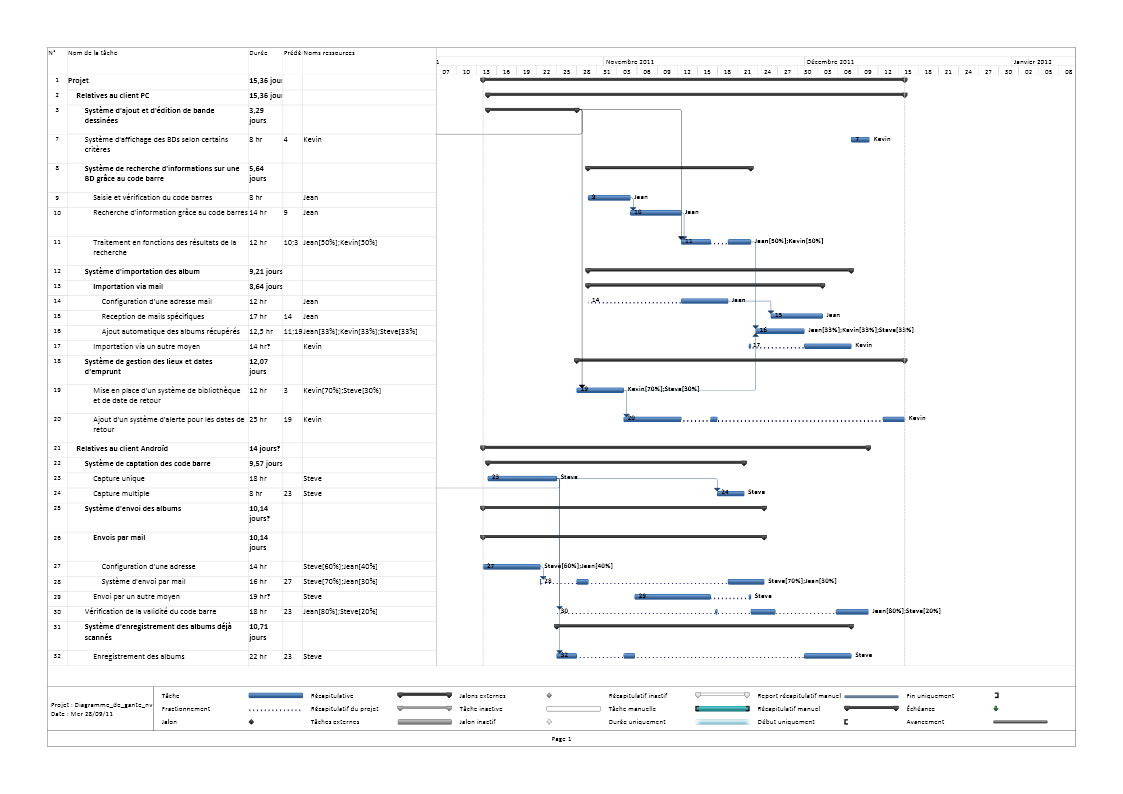
\includegraphics[width=15cm]{../Diagramme_gante.png}
\end{wrapfigure}
\clearpage

\subsection{Comparaison des méthodes}
\emph{Microsoft Project} a caculé un temps de développement de \textbf{253h}. 
Avec notre estimation par analogie, nous avons trouvé un temps consacré au développement de \textbf{300h}. 
Nous pouvons donc dire que globalement, les résultats concordent. 
Ceux-ci peuvent donc être fiables, et le temps réel devrait se situer entre 253 et 300h de codage. 

\subsection{Difficultés encourues} 
L'estimation du temps de réalisation des fonctionnalités à été un problème. 
En effet, le manque d'expérience dans le domaine du travail en équipe nous empêche de bien définir si nos enchainements entre la réalisation des fonctionnalités se dérouleront bien comme prévu, et si nous arriverons à travailler ensemble efficacement. 

Le deuxième problème dans l'estimation vient de notre manque d'expérience en tant que programmeur :
L'instabilité des connaissances acquises nous fera peut-être perdre du temps dans l'apprentissage de quelque chose qu'on aura estimé plus simple à assimiler. 

\newpage{}

\part{Définition des contraintes}


\section{Contraintes de temps}
Pour notre projet nous avons un temps imparti avec au moins trois étapes donc au moins trois livrables. Ces remises ne nous permettent aucuns retard donc chaque étape du projet devra être terminée dans les temps impartis.
Les autres contraintes de temps que nous pourront rencontrer lors de ce projet sont les heures que l'on devra consacrer à nos études de façon extérieure au projet (par exemple pendant les partiels). 

\section{Contraintes de qualités}

\subsection{Charte ergonomique}
Notre projet étant l'amélioration d'un programme déjà existant nous aurons à respecter la charte graphique déjà existante afin de concorder avec le reste du programme. 
De même, pour l'application Androïd, nous aurons à nous adapter à une utilisation tactile de l'application. 

\subsection{Norme d'écriture}
Royal est un projet open - source. 
Nous nous devons de redistribuer le code source qu'on créera.
Pour ce fait, des normes d'écritures doivent êtres mise en place afin de faciliter la compréhension de notre code par d'autres personnes susceptible de reprendre le projet. 
Nous devrons également écrire les commentaires dans notre programme en anglais, comme c'est le cas dans Royal à présent.

\section{Contraintes matérielles et technologiques}

\subsection{Adaptation aux outils utilisés dans Royal}
Pour notre projet nous devons nous adapter au outils déjà utilisés. Une bonne partie de notre travail consistera à comprendre le fonctionnement de ces outils.

\subsection{Compatibilité du client lourd}
Le client lourd devra pouvoir s'installer sous Linux et si possible sur Windows et MacOS. 
Pour permettre cette comptabilité nous devrons veiller à fournir les différentes librairies adaptées aux différents systèmes d'exploitation avec notre programme. 

\subsection{Compatibilité du client mobile}
L'application mobile devra être compatible avec les téléphones Androïd à partir de la version 2.2. 
Nous devrons aussi faire attention à ce que les différentes librairies utilisées soient déjà installées sur le téléphone, ou dans le cas contraire les installer automatiquement.

\section{Contraintes de realisation}

\subsection{Designation des acteurs}
Pour ce projet notre maître d'ouvrage est Maitre Ogier, pour ce qui est des maître d'oeuvre notre équipe est composée de Hagner Kévin le chef de projet, Meyblum Jean ainsi que Benedick Steve.
Afin pour faciliter la communication entre notre tuteur et nous, nous avons choisi d'organiser des réunions une à deux fois par semaine. De même Maitre Ogier pourra suivre le développement de notre projet sur notre dépot Git.
\footnote{Page Github de notre depot Git: https://github.com/spydemon/Royal\_} 
Pour ce qui est de la communication entre les membres de notre trinôme nous avons crée un canal irc \footnote{ canal \#royal\_ sur le serveur irc.rezosup.org} afin de pouvoir faciliter la discution à plusieurs. 
De même nous pourrons travailler ensemble soit a l'IUT soit chez l'un des membres si besoin.

\subsection{Cycle de vie}
Afin de développer parallèlement différents modules une fois la phase notre cahier des charge validé nous avons choisi un cycle de vie en W. 
En effet comme dans ce modèle l'intégration est déja étudiée lors de la conception globale des fonctionnalités nous pouvons concevoir, développer et tester chaque fonctionnalitée séparément. 
De même ce cycle de vie nous permet de développer notre projet en fonction des priorités de nos tâches ce qui nous permet de garantir au minimum le rendu d'un projet répondant aux demandes de base.


\end{document}
